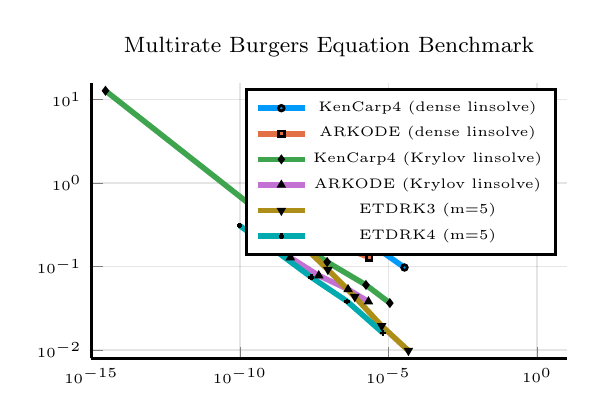
\begin{tikzpicture}[]
\begin{axis}[height = {50.8mm}, title = {Multirate Burgers Equation Benchmark}, xmin = {1.0e-15}, xmax = {10}, ymax = {15.776844127916583}, ymode = {log}, unbounded coords=jump,scaled x ticks = false,xlabel style = {font = {\fontsize{5 pt}{6.5 pt}\selectfont}, color = {rgb,1:red,0.00000000;green,0.00000000;blue,0.00000000}, draw opacity = 1.0, rotate = 0.0},log basis x=10,xmajorgrids = true,xtick = {1.0e-15,1.0e-10,1.0e-5,1.0},xticklabels = {$10^{-15}$,$10^{-10}$,$10^{-5}$,$10^{0}$},xtick align = inside,xticklabel style = {font = {\fontsize{5 pt}{6.5 pt}\selectfont}, color = {rgb,1:red,0.00000000;green,0.00000000;blue,0.00000000}, draw opacity = 1.0, rotate = 0.0},x grid style = {color = {rgb,1:red,0.00000000;green,0.00000000;blue,0.00000000},
draw opacity = 0.1,
line width = 0.5,
solid},axis lines* = left,x axis line style = {color = {rgb,1:red,0.00000000;green,0.00000000;blue,0.00000000},
draw opacity = 1.0,
line width = 1,
solid},scaled y ticks = false,ylabel style = {font = {\fontsize{5 pt}{6.5 pt}\selectfont}, color = {rgb,1:red,0.00000000;green,0.00000000;blue,0.00000000}, draw opacity = 1.0, rotate = 0.0},log basis y=10,ymajorgrids = true,ytick = {0.01,0.1,1.0,10.0},yticklabels = {$10^{-2}$,$10^{-1}$,$10^{0}$,$10^{1}$},ytick align = inside,yticklabel style = {font = {\fontsize{5 pt}{6.5 pt}\selectfont}, color = {rgb,1:red,0.00000000;green,0.00000000;blue,0.00000000}, draw opacity = 1.0, rotate = 0.0},y grid style = {color = {rgb,1:red,0.00000000;green,0.00000000;blue,0.00000000},
draw opacity = 0.1,
line width = 0.5,
solid},axis lines* = left,y axis line style = {color = {rgb,1:red,0.00000000;green,0.00000000;blue,0.00000000},
draw opacity = 1.0,
line width = 1,
solid},    xshift = 0.0mm,
    yshift = 0.0mm,
    axis background/.style={fill={rgb,1:red,1.00000000;green,1.00000000;blue,1.00000000}}
,title style = {font = {\fontsize{8 pt}{10.4 pt}\selectfont}, color = {rgb,1:red,0.00000000;green,0.00000000;blue,0.00000000}, draw opacity = 1.0, rotate = 0.0},legend style = {color = {rgb,1:red,0.00000000;green,0.00000000;blue,0.00000000},
draw opacity = 1.0,
line width = 1,
solid,fill = {rgb,1:red,1.00000000;green,1.00000000;blue,1.00000000},font = {\fontsize{3 pt}{3.9000000000000004 pt}\selectfont}},colorbar style={title=}, xmode = {log}, ymin = {0.007904077109128715}, width = {76.2mm}]\addplot+ [color = {rgb,1:red,0.00000000;green,0.60560316;blue,0.97868012},
draw opacity = 1.0,
line width = 2,
solid,mark = *,
mark size = 1.0,
mark options = {
    color = {rgb,1:red,0.00000000;green,0.00000000;blue,0.00000000}, draw opacity = 1.0,
    fill = {rgb,1:red,0.00000000;green,0.60560316;blue,0.97868012}, fill opacity = 1.0,
    line width = 1,
    rotate = 0,
    solid
}]coordinates {
(3.4648103383872526e-5, 0.097071093)
(2.7814951199546194e-6, 0.181906111)
(2.118105787153261e-7, 0.341356229)
(2.0098094007543837e-8, 0.631136249)
(1.959516371706548e-9, 1.086916523)
};
\addlegendentry{KenCarp4 (dense linsolve)}
\addplot+ [color = {rgb,1:red,0.88887350;green,0.43564919;blue,0.27812294},
draw opacity = 1.0,
line width = 2,
solid,mark = square*,
mark size = 1.0,
mark options = {
    color = {rgb,1:red,0.00000000;green,0.00000000;blue,0.00000000}, draw opacity = 1.0,
    fill = {rgb,1:red,0.88887350;green,0.43564919;blue,0.27812294}, fill opacity = 1.0,
    line width = 1,
    rotate = 0,
    solid
}]coordinates {
(2.2707765343744006e-6, 0.128150168)
(3.6788876697267834e-7, 0.164177227)
(4.455204624858925e-8, 0.234420187)
(5.352076989144092e-9, 0.364909279)
(5.35662117817959e-10, 0.597057398)
};
\addlegendentry{ARKODE (dense linsolve)}
\addplot+ [color = {rgb,1:red,0.24222430;green,0.64327509;blue,0.30444865},
draw opacity = 1.0,
line width = 2,
solid,mark = diamond*,
mark size = 1.0,
mark options = {
    color = {rgb,1:red,0.00000000;green,0.00000000;blue,0.00000000}, draw opacity = 1.0,
    fill = {rgb,1:red,0.24222430;green,0.64327509;blue,0.30444865}, fill opacity = 1.0,
    line width = 1,
    rotate = 0,
    solid
}]coordinates {
(1.113318376312209e-5, 0.036404373)
(1.7477558362010042e-6, 0.060001805)
(8.624006797682366e-8, 0.113135202)
(6.321267939163031e-9, 0.215084504)
(2.9957635733888373e-15, 12.72386716)
};
\addlegendentry{KenCarp4 (Krylov linsolve)}
\addplot+ [color = {rgb,1:red,0.76444018;green,0.44411178;blue,0.82429754},
draw opacity = 1.0,
line width = 2,
solid,mark = triangle*,
mark size = 1.0,
mark options = {
    color = {rgb,1:red,0.00000000;green,0.00000000;blue,0.00000000}, draw opacity = 1.0,
    fill = {rgb,1:red,0.76444018;green,0.44411178;blue,0.82429754}, fill opacity = 1.0,
    line width = 1,
    rotate = 0,
    solid
}]coordinates {
(2.118411571520636e-6, 0.037960327)
(4.373166746363195e-7, 0.053110761)
(4.5087873239683744e-8, 0.077791497)
(4.9772815346311464e-9, 0.127812883)
(5.193626980967097e-10, 0.2114173)
};
\addlegendentry{ARKODE (Krylov linsolve)}
\addplot+ [color = {rgb,1:red,0.67554396;green,0.55566233;blue,0.09423434},
draw opacity = 1.0,
line width = 2,
solid,mark = triangle*,
mark size = 1.0,
mark options = {
    color = {rgb,1:red,0.00000000;green,0.00000000;blue,0.00000000}, draw opacity = 1.0,
    fill = {rgb,1:red,0.67554396;green,0.55566233;blue,0.09423434}, fill opacity = 1.0,
    line width = 1,
    rotate = 180,
    solid
}]coordinates {
(4.693599813090348e-5, 0.009800589)
(5.914208264839906e-6, 0.019406029)
(7.360331501650721e-7, 0.043309185)
(9.167567766999955e-8, 0.091419605)
(1.1435992218461219e-8, 0.187469357)
};
\addlegendentry{ETDRK3 (m=5)}
\addplot+ [color = {rgb,1:red,0.00000048;green,0.66575898;blue,0.68099695},
draw opacity = 1.0,
line width = 2,
solid,mark = +,
mark size = 1.0,
mark options = {
    color = {rgb,1:red,0.00000000;green,0.00000000;blue,0.00000000}, draw opacity = 1.0,
    fill = {rgb,1:red,0.00000048;green,0.66575898;blue,0.68099695}, fill opacity = 1.0,
    line width = 1,
    rotate = 0,
    solid
}]coordinates {
(6.535650828647287e-6, 0.015969848)
(4.054496929215464e-7, 0.038185714)
(2.5120547006198278e-8, 0.074337009)
(1.5617106897893295e-9, 0.154802398)
(9.732799825817218e-11, 0.308371751)
};
\addlegendentry{ETDRK4 (m=5)}
\end{axis}

\end{tikzpicture}
